% !TEX root = main.tex
% --+ 11.51 SUMMARY +-----------------------------------------------------------
\begin{frame}{Acceptance Correction: Generation + Simulation}
    \label{11.51::summary}
    \begin{itemize}
        \item
            To apply acceptance correction, 10M DIS events were generated in \ef{LEPTO}.

        \item
            Then, they were simulated with \ef{GEMC 5.2} with run 12016's conditions.

        \item
            Finally, they were reconstructed with \ef{Coatjava 8.2.0}.
    \end{itemize}

    \vspace{-12pt}

    \begin{columns}[onlytextwidth,T]

    \begin{column}{.05\linewidth}\end{column} % Centering column.

    \begin{column}{.35\linewidth}
        \begin{center}
            \begin{figure}[t]
                \centering{
                    \fbox{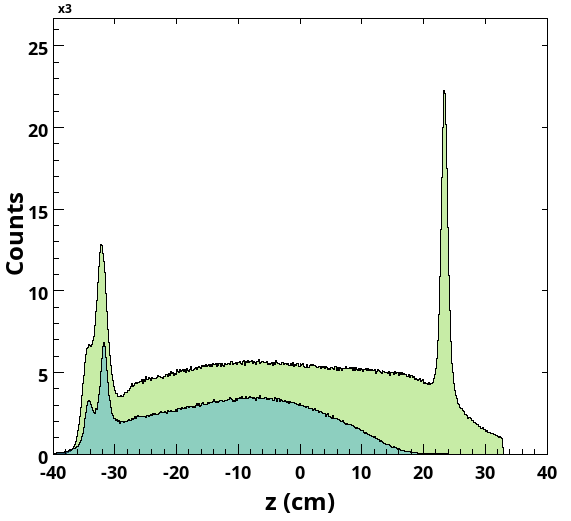
\includegraphics[width=\textwidth]{51vz_012016.png}}
                }
                \textit{Run \ef{12016}.}
            \end{figure}
        \end{center}
    \end{column}

    \begin{column}{.35\linewidth}
        \begin{center}
            \begin{figure}[t]
                \centering{
                    \fbox{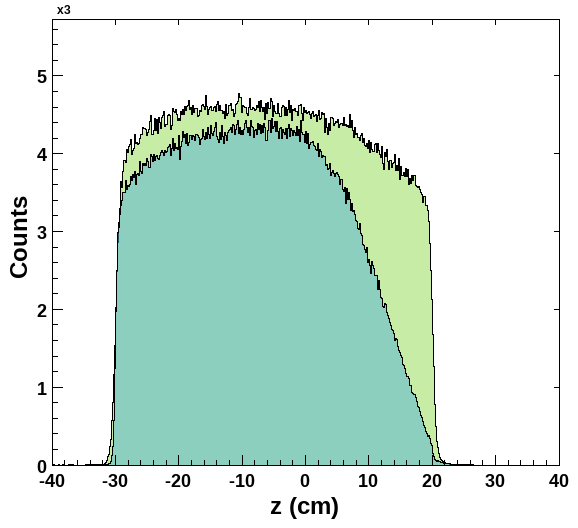
\includegraphics[width=\textwidth]{51vz_999106.png}}
                }
                \textit{Simulated data.}
            \end{figure}
        \end{center}
    \end{column}

    \begin{column}{.05\linewidth}\end{column} % Centering column.

    \end{columns}

    \begin{center}
        \textit{\ef{$v_z$} for \textbf{\textcolor[HTML]{c7eca6}{DC (green)}} and \textbf{\textcolor[HTML]{8dcfbf}{FMT (cyan)}} tracks}
    \end{center}
\end{frame}

